\documentclass[11pt]{article}
\usepackage{homework}

\classname{364}
\homeworknum{4}

\DeclareMathAlphabet{\mathsfit}{T1}{\sfdefault}{\mddefault}{\sldefault}


\begin{document}

% Environments

\newcommand{\state}[2]{\begin{statement}{#1} #2 \end{statement}}
\newcommand{\prob}[2]{\begin{problem}{#1} #2 \end{problem}}
\newcommand{\subprob}[1]{\begin{subproblem} #1 \end{subproblem}}
\newcommand{\sol}[1]{\begin{solution} #1 \end{solution}}
\newcommand{\fig}[2]{\begin{figure} \centering #2  \label{#1} \end{figure}}

\newcommand{\makebib}{
	\vfill
	\color{black}
	\nocite{*}
	\bibliography{references}{}
	\bibliographystyle{lucas_unsrt}
}
	

% Implication

\newcommand{\qwhere}{\quad \text{where} \quad}
\newcommand{\qimplies}{\quad \implies \quad}
\newcommand{\impliesq}{\implies \quad}



% Brackets

\newcommand{\paren}[1]{\left( #1 \right)}
\newcommand{\brac}[1]{\left[ #1 \right]}
\newcommand{\curly}[1]{\left\{ #1 \right\}}


% Greek

\newcommand{\alp}{\alpha}
\newcommand{\bet}{\beta}
\newcommand{\gam}{\gamma}
\newcommand{\del}{\delta}
\newcommand{\eps}{\epsilon}
\newcommand{\zet}{\zeta}
\newcommand{\tht}{\theta}
\newcommand{\kap}{\kappa}
\newcommand{\lam}{\lambda}
\newcommand{\sig}{\sigma}
\newcommand{\ups}{\upsilon}
\newcommand{\omg}{\omega}

\newcommand{\Gam}{\Gamma}
\newcommand{\Del}{\Delta}
\newcommand{\Tht}{\Theta}
\newcommand{\Lam}{\Lambda}
\newcommand{\Sig}{\Sigma}
\newcommand{\Omg}{\Omega}


% Text

\newcommand{\where}{\text{where }}

% Problem 1

\newcommand{\Hint}{H_\text{int}}
\newcommand{\ddcx}{\dd[3]{x}}
\newcommand{\psib}{\bar{\psi}}

\newcommand{\mh}{m_h}
\newcommand{\mmu}{m_\mu}
\newcommand{\me}{m_e}
\newcommand{\ma}{m_a}

\newcommand{\aexpt}{a_\text{expt.}}
\newcommand{\aQED}{a_\text{QED}}
\renewcommand{\GeV}{\giga\electronvolt}

\newcommand{\gamt}{\gam^5}

\state{}{
	Consider a particle which, as viewed by an observer in an inertial lab, is in a circular orbit in the $(x, y)$ plane with angular velocity $\omg$ and radius $r$.  Suppose that this particle carries a spin angular momentum $\vS$ (treated classically in this problem) which is Fermi-Walker transported.  Compute the time dependence of this angular momentum $\vSt$ where $t$ is the inertial time in the laboratory frame.  Show that in the non-relativistic limit, the complex vector $\Sx + i \Sy$ precesses about the $z$ axis with frequency $\omgT = r^2 \omg^3 / 2$.
}

\sol{
	Since the particle is in a circular orbit in the $xy$ plane, we can write its position in the lab frame as
	\eq{
		\vx = ( t, r \cos(\omg t), r \sin(\omg t), 0 ).
	}
	Then from MCP~(2.7), its velocity is
	\eqn{U}{
		\vU = \dv{\vx}{\tau}
		= \gam ( 1, -r \omg \sin(\omg t), r \omg \cos(\omg t), 0 ),
	}
	since $\ddtau = \ddt / \gam$~\cite[p.~201]{Resnick}.  The particle's acceleration is
	\eq{
		\vaa = \dv{\vU}{\tau}
		= -r \omg^2 \gam^2 ( 0, \cos(\omg t), \sin(\omg t), 0 ).
	}
	The Fermi-Walker transport is, as given by MCP~(24.62),
	\eqn{FW}{
		\nabsU \vS = \vU (\vaa \cdot \vS),
	}
	and we know that the spin vector is always orthogonal to the particle's 4-velocity~\cite[p.~1184]{MCP}.  This means that the spin vector can be written
	\eq{
		\vS = (0, \bS)
	}
	since $\vU \cdot \vS = 0$ is Lorentz invariant, and the spatial components of the particle's velocity are zero in its rest frame.  Moreover, this means
	\eq{
		\nabsU \vS = -\dv{\vS}{\tau}
		= -\gam \dv{\vS}{t},
	}
	so Eq.~\refeq{FW} can be written
	\eq{
		\dv{\vS}{t} = -\frac{1}{\gam} \vU (\vaa \cdot \vS)
		= \gam r \omg^2 [ \Sx \cos(\omg t) + \Sy \sin(\omg t) ] \vU.
	}
	Feeding in the relevant components of Eq.~\refeq{U}, we have the system of coupled differential equations
	\al{
		\dv{\Sx}{t} &= -\gam^2 r^2 \omg^3 \sin(\omg t) [ \Sx \cos(\omg t) + \Sy \sin(\omg t) ], \\
		\dv{\Sy}{t} &= \gam^2 r^2 \omg^3 \cos(\omg t) [ \Sx \cos(\omg t) + \Sy \sin(\omg t) ],
	}
	or, in matrix form,
	\eqn{sysxy}{
		\dv{t} \mqty[ \Sx \\ \Sy ] = \gam^2 r^2 \omg^3 \mqty[
				-\cos(\omg t) \sin(\omg t) & -\sin[2](\omg t) \\
				\cos[2](\omg t) & \cos(\omg t) \sin(\omg t)
			] \mqty[ \Sx \\ \Sy ].
	}
	To solve the system, we define the polar components of $\vS$ by~\cite[inside cover]{Griffiths}
	\al{
		\Sr &= \Sx \cos(\omg t) + \Sy \sin(\omg t), &
		\Stht &= -\Sx \sin(\omg t) + \Sy \cos(\omg t).
	}
	Then we can transform into these polar coordinates using the matrix~\cite[inside cover]{Griffiths}
	\eqn{sub1}{
		\mqty[ \Sx \\ \Sy ] = \mqty[
				\cos(\omg t) & -\sin(\omg t) \\
				\sin(\omg t) & \cos(\omg t)
			] \mqty[ \Sr \\ \Stht ],
	}
	which implies
	\aln{
		\dv{t} \mqty[ \Sx \\ \Sy ] &= \dv{t} \mqty[
				\cos(\omg t) & -\sin(\omg t) \\
				\sin(\omg t) & \cos(\omg t)
			] \mqty[ \Sr \\ \Stht ] + \mqty[
				\cos(\omg t) & -\sin(\omg t) \\
				\sin(\omg t) & \cos(\omg t)
			] \dv{t} \mqty[ \Sr \\ \Stht ] \\ \notag
		&= -\omg \mqty[
			\sin(\omg t) & \cos(\omg t) \\
			-\cos(\omg t) & \sin(\omg t)
		] \mqty[ \Sr \\ \Stht ] + \mqty[
				\cos(\omg t) & -\sin(\omg t) \\
				\sin(\omg t) & \cos(\omg t)
			] \dv{t} \mqty[ \Sr \\ \Stht ]. \label{sub2}
	}
	Substituting Eqs.~\refeq{sub1} and \refeq{sub2} into Eq.~\refeq{sysxy} yields
	\al{
		-\omg &\mqty[
				\sin(\omg t) & \cos(\omg t) \\
				-\cos(\omg t) & \sin(\omg t)
			] \mqty[ \Sr \\ \Stht ] + \mqty[
				\cos(\omg t) & -\sin(\omg t) \\
				\sin(\omg t) & \cos(\omg t)
			] \dv{t} \mqty[ \Sr \\ \Stht ] \\
		&\hspace{10em} = \gam^2 r^2 \omg^3 \mqty[
				-\cos(\omg t) \sin(\omg t) & -\sin[2](\omg t) \\
				\cos[2](\omg t) & \cos(\omg t) \sin(\omg t)
			] \mqty[
				\cos(\omg t) & -\sin(\omg t) \\
				\sin(\omg t) & \cos(\omg t)
			] \mqty[ \Sr \\ \Stht ] \\
		&\hspace{10em} = \gam^2 r^2 \omg^3 \mqty[
				-\sin(\omg t) & 0 \\
				\cos(\omg t) & 0
			] \mqty[ \Sr \\ \Stht ],
	}
	where the matrix multiplication has been carried out with Mathematica.  This implies
	\al{
		\mqty[
				\cos(\omg t) & -\sin(\omg t) \\
				\sin(\omg t) & \cos(\omg t)
			] \dv{t} \mqty[ \Sr \\ \Stht ]
		&= \paren{ \omg \mqty[
				\sin(\omg t) & \cos(\omg t) \\
				-\cos(\omg t) & \sin(\omg t)
			] + \gam^2 r^2 \omg^3 \mqty[
				-\sin(\omg t) & 0 \\
				\cos(\omg t) & 0
			] } \mqty[ \Sr \\ \Stht ] \\
		&= \omg \mqty[
				(1 - \gam^2 r^2 \omg^2) \sin(\omg t) & \cos(\omg t) \\
				-(1 - \gam^2 r^2 \omg^2) \cos(\omg t) & \sin(\omg t)
			] \mqty[ \Sr \\ \Stht ].
	}
	Multiplying both sides by the inverse of the first matrix, we find
	\eq{
		\dv{t} \mqty[ \Sr \\ \Stht ] = \omg \mqty[
				\cos(\omg t) & \sin(\omg t) \\
				-\sin(\omg t) & \cos(\omg t)
			] \mqty[
				(1 - \gam^2 r^2 \omg^2) \sin(\omg t) & \cos(\omg t) \\
				-(1 - \gam^2 r^2 \omg^2) \cos(\omg t) & \sin(\omg t)
			] \mqty[ \Sr \\ \Stht ]
		= \omg \mqty[
				0 & 1 \\
				\gam^2 r^2 \omg^2 - 1 & 0
			] \mqty[ \Sr \\ \Stht ].
	}
	In other words, we have a system of coupled first-order ODEs:
	\aln{ \label{ODEs}
		\dv{\Sr}{t} &= \omg \Stht, &
		\dv{\Stht}{t} &= \omg (\gam^2 r^2 \omg^2 - 1) \Sr.
	}
%	However, we know that $\Sr(t) = S = \const$, since the magnitude of the spin should not change with time.  Let $\alp \equiv \omg^2 (\gam^2 r^2 \omg^2 - 1)$.  Then, imposing the initial condition $\Stht(0) = 0$,
%	\al{
%		\Sr(t) &= S, &
%		\Stht(t) &= \alp S t.
%	}
%	Now we use Eq.~\refeq{sub1} to transform back to Cartesian components:
%	\al{
%		\Sx(t) &= S \cos(\omg t) - \alp S \sin(\omg t) t
%	}
%	
%	\hl{actually this doesn't make sense}
%
	Differentiating each equation by $t$ once more and substituting, we get a system of uncoupled second-order ODEs with well-known solutions:
	\al{
		\dv[2]{\Sr}{t} &= \omg \dv{\Stht}{t}
		= \omg^2 (\gam^2 r^2 \omg^2 - 1) \Sr, &
		%
		\dv[2]{\Stht}{t} &= \omg (\gam^2 r^2 \omg^2 - 1) \dv{\Sr}{t}
		= \omg^2 (\gam^2 r^2 \omg^2 - 1) \Stht.
	}
	Let $\alp \equiv \omg^2 (\gam^2 r^2 \omg^2 - 1)$.  Then the solutions are~\cite[p.~207]{Swartz}
	\al{
		\Sr(t) &= \Cq \cos(-\alp t) + \Cw \sin(-\alp t), &
		\Stht(t) &= \Dq \cos(-\alp t) + \Dw \sin(-\alp t).
	}
	We transform back into Cartesian components via Eq.~\refeq{sub1}:
	\al{
		\mqty[ \Sx \\ \Sy ] &= \mqty[
				\cos(\omg t) & -\sin(\omg t) \\
				\sin(\omg t) & \cos(\omg t)
			] \mqty[ 
				\Cq \cos(-\alp t) + \Cw \sin(-\alp t) \\
				\Dq \cos(-\alp t) + \Dw \sin(-\alp t)
			] \\
		&= \mqty[
				\cos(\omg t) [ \Cq \cos(-\alp t) + \Cw \sin(-\alp t) ] - \sin(\omg t) [ \Dq \cos(-\alp t) + \Dw \sin(-\alp t) ] \\
				\sin(\omg t) [ \Cq \cos(-\alp t) + \Cw \sin(-\alp t) ] + \cos(\omg t) [ \Dq \cos(-\alp t) + \Dw \sin(-\alp t) ].
			]
	}
	We choose the initial conditions $\Sx(0) = S$, $\Sy(0) = 0$, which give us
	\al{
		\Sx(0) &= S
		= \Cq, &
		%
		\Sy(0) &= 0
		= \Dq.
	}
	Using these results and the initial conditions in Eq.~\refeq{sysxy}, we have
	\eq{
		\left. \dv{t} \mqty[ \Sx \\ \Sy ] \right|_{t = 0} = \gam^2 r^2 \omg^3 \mqty[
				0 & 0 \\
				1 & 0
			] \mqty[
				S \\
				0
			]
		= \gam^2 r^2 \omg^3 \mqty[ 0 \\ S ],
	}
	with
	\eq{
		\left. \dv{t} \mqty[ \Sx \\ \Sy ] \right|_{t = 0} = 
	}
	\hl{but this is getting really gross}
	
	\eq{
		\mqty[ \Sx \\ \Sy ] = \mqty[
				\cos(\omg t) [ S \cos(-\alp t) + \Cw \sin(-\alp t) ] - \Dw \sin(\omg t) \sin(-\alp t) \\
				\sin(\omg t) [ S \cos(-\alp t)  + \Cw \sin(-\alp t) ] + \Dw \cos(\omg t) \sin(-\alp t)
			]
	}
	\eq{
		\mqty[ 0 \\ S ](t = -\pi \alp / 2) = \mqty[
				\Cw \cos(-\pi \omg \alp / 2) - \Dw \sin(-\pi \omg \alp / 2) \\
				\Cw \sin(-\pi \omg \alp / 2) + \Dw \cos(-\pi \omg \alp / 2)
			]
	}
	
	
%	We choose the initial conditions $\Sr(0) = S$ and $\Stht(0) = 0$.  This gives us
%	\al{
%		S &= \Sr(0) = \Cq, &
%		0 &= \Stht(0) = \Dq.
%	}
%	Then by Eq.~\refeq{ODEs},
%	\al{
%		\omg \Dw \sin(-\alp t) &= \dv{\Sr}{t} = \omg \alp [ S \sin(-\alp t) - \Cw \cos(-\alp t) ], \\
%		\omg \alp [ S \cos(-\alp t) + \Cw \sin(-\alp t) ] &= \dv{\Stht}{t} = -\alp \Dw \cos(-\alp t)
%	}
}





\clearpage
\state{Gravitational redshift~(MCP 24.16)}{
	Inside a laboratory on Earth's surface the effects of spacetime curvature are so small that current technology cannot measure them.  Therefore, experiments performed in the laboratory can be analyzed using special relativity. %  (This fact is embodied in Einstein's equivalence principle.)
}

\prob{
	Explain why the spacetime metric in the proper reference frame of the laboratory's floor has the form
	\eqn{metric2}{
		\dds^2 = (1 + 2 g z) (\ddxoh)^2 + \ddx^2 + \ddy^2 + \ddz^2,
	}
	plus terms due to the slow rotation of the laboratory walls, which we neglect in this exercise.  Here $g$ is the acceleration of gravity measured on the floor.
}

\sol{
	We can transform coordinates from the proper reference frame of the laboratory floor to another inertial frame.  We choose this other frame such that it is only a very small ``distance'' away at $\vx = 0$ in the proper frame.  That is, the frames are identical in the immediate vicinity of event (small $\vx$).  Then the coordinate transformation from the proper reference frame to the other inertial frame is given by MCP~(24.60a),
	\al{
		\xii &= \xiih + \frac{1}{2} \aih (\xoh)^2 + \epsisjkh \Omgjh \xkh \xoh, &
		\xo &= \xoh (1 + \asjh \xjh),
	}
	where terms to quadratic order in $\xah$ are included, and $\Omgjh$ is the rotational angular velocity of the laboratory.  Since the metric in the inertial frame is $\dds^2 = -(\ddxo)^2 + \delsij \ddxii \ddxj$~\cite[p.~1183]{MCP}, the metric in the proper reference frame is given by MCP~(24.60b),
	\eq{
		\dds^2 = -(1 + 2 \ba \vdot \bx) (\ddxoh)^2 + 2 (\bOmg \cross \bx) \vdot \ddbx \ddxoh + \delsjk \ddxjh \ddxkh,
	}
	which is accurate to linear order in $\xah$.  For this problem, we ignore rotations so $\bOmg \to \bo$, eliminating the second term.  Also, $\ba = g \zh$ so $\ba \vdot \bx = -g z$.  Finally, we note that $\xiih \in \{ x, y, z \}$ since these coordinates coincide with the inertial frame~\cite[p.~1186]{MCP}.  Then the spacetime metric is
	\eq{
		\dds^2 = -(1 + 2 g z) (\ddxoh)^2 + \ddx^2 + \ddy^2 + \ddz^2,
	}
	which is what we want.  Evidently, there is a typo (missing minus sign) in the problem statement. \qed
}


\prob{
	An electromagnetic wave is emitted from the floor, where it is measured to have wavelength $\lamo$, and is received at the ceiling.  Using the metric of Eq.~\refeq{metric2}, show that, as measured in the proper reference frame of an observer on the ceiling, the received wave has wavelength $\lamr = \lamo (1 + g h)$, where $h$ is the height of the ceiling above the floor (i.e., the light is \emph{gravitationally redshifted} by $\Del\lam / \lamo = g h$).
	
	Hint: Show that all crests of the wave must travel along world lines that have the same shape, $z = F(\xoh - \xohe)$, where $F$ is some function, and $\xohe$ is the coordinate time at which the crest is emitted from the floor. %  You can compute the shape function $F$ if you wish, but it is not needed to derive the gravitational redshift; only its universality is needed.]
}





\clearpage
\state{Rigidly rotating disk~(MCP 24.17)}{
	Consider a thin disk with radius $R$ at $z = 0$ in a Lorentz reference frame.  The disk rotates rigidly with angular velocity $\Omg$.  In the early years of special relativity there was much confusion over the geometry of the disk: In the inertial frame it has physical radius (proper distance from center to edge) $R$ and physical circumference $\sC = 2\pi R$.  But Lorentz contraction dictates that, as measured on the disk, the circumference should be $\sqrt{1 - v^2} \sC$ (with $v = \Omg R$), and the physical radius, $R$, should be unchanged.  This seemed weird.  How could an obviously flat disk in spacetime have a curved, non-Euclidean geometry, with physical circumference divided by physical radius smaller than $2\pi$?  In this exercise you will explore this issue.
}

\prob{
	Consider a family of observers who ride on the edge of the disk.  Construct a circular curve, orthogonal to their world lines, that travels around the disk (at $\sqrt{x^2 + y^2} = R$).  This curve can be thought of as lying in a 3-surface of constant time $\xoh$ of the observers' proper reference frames.  Show that it spirals upward in a Lorentz-frame spacetime diagram, so it cannot close on itself after traveling around the disk.  Thus the 3-planes, orthogonal to the observers' world lines at the edge of the disk, cannot mesh globally to form global 3-planes.
}

%\sol{
%	Each observer has a helical worldline.  If we flatten the worldline into one spatial and one temporal dimension, it looks like a sinusoid.  A spacetime diagram for a family of three observers riding on the edge of the disk is shown in Fig.~\ref{f3a}.  Here we have chosen $v = 0.5$, and show approximately six cycles.  In the figure, the $y$ axis points directly into the page.  The father, whose worldline is drawn in blue, has the initital position $(x, y) = (0, R)$ at $t = 0$.  The mother~(red worldline) begins at $(R, 0)$ and their child~(violet worldline) at $(R / \sqrt{2}, R / \sqrt{2})$.  The gray line is the circular curve orthogonal to their worldlines.  This curve is helical, like the worldlines, but with opposite chirality and a far steeper pitch.  Since it is a helix, it does not close on itself after one complete rotation. \qed
%	
%	\begin{figure} \centering
%		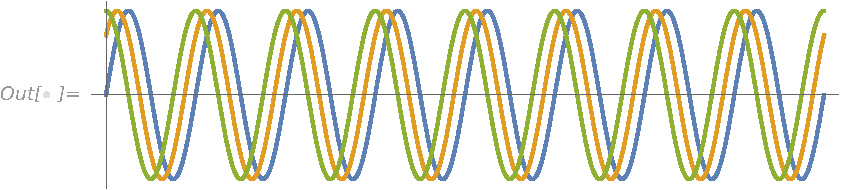
\includegraphics[angle=90,origin=c,trim=1.5cm 0 0 0,clip]{3a}
%		\bigskip
%		\caption{Spacetime diagram for a family of three observers riding on the edge of the disk.  The $y$ axis points directly into the page.  The blue, red, and violet lines are the worldlines of the family members, and the gray line is orthogonal to them.} 
%		\label{f3a}
%	\end{figure}
%}



\prob{
	Next, consider a 2-dimensional family of observers who ride on the surface of the rotating disk.  Show that at each radius $\sqrt{x^2 + y^2} = \const$, the constant-radius curve that is orthogonal to their world lines spirals upward in spacetime with a different slope.  Show that this means that even locally, the 3-planes orthogonal to each of their world lines cannot mesh to form larger 3-planes---thus there does not reside in spacetime any 3-surface orthogonal to these observers' world lines.  There is no 3-surface that has the claimed non-Euclidean geometry.
}

%\sol{
%	Now we consider the case in which all three observers have the same phase $\phi = 0$, but different radii.  In nonrelativistic rotation, the sinusoids would differ only by their amplitude.  In this case, however, the periods are not the same at different radii, since the circumference depends on velocity, which in turn depends on the radius.  The larger the radius, the 
%	
%	Figure~\ref{f3b1} shows the worldlines of the observers in this case; the father's blue worldline has radius $R$, the mother's red worldline has radius $R/3$, and the child's violet worldline has radius $2R / 3$.  (The $t$ axis is zoomed in with respect to Fig.~\ref{f3a}.)  The closer the worldline is to the edge of the disk, the greater the velocity, 
%	
%	 Figure~\ref{f3b1} shows the same worldlines, but with the amplitudes normalized to better compare the pitch of the helices  Figure~\ref{f3b1} shows
%	 
%	 
%	 \hl{actually idk wtf is going on}
%}






\clearpage
\state{Constant of geodesic motion in a spacetime with symmetry~(MCP 25.4)}{\hfix}

\prob{
	Suppose that in some coordinate system the metric coefficients are independent of some specific coordinate $\xA$: $\sgsabA = 0$ (e.g., in spherical polar coordinates $\{ t, r, \tht, \phi \}$ in flat spacetime $\sgsabphi = 0$, so we could set $\xA = \phi$).  Show that
	\eq{
		\psA \equiv \vp \cdot \pdv{\xA}
	}
	is a constant of the motion for a freely moving particle [$\psp = (\text{conserved $z$~component of angular momentum})$] in the above, spherically symmetric example.]
	
	Hint: Show that the geodesic equation can be written in the form
	\eq{
		\dv{\psa}{\zet} - \Gamsman \pmu \pnu = 0,
	}
	where $\Gamsman$ is the covariant connection of Eqs.~(24.38c), (24.38d) with $\csabg = 0$, because we are using a coordinate basis.
	
	Note the analogy of the constant of motion $\psA$ with Hamiltonian mechanics; there, if the Hamiltonian is independent of $\xA$, then the generalized momentum $\psA$ is conserved; here, if the metric coefficients are independent of $\xA$, then the covariant component $\psA$ of the momentum is conserved.
}



\prob{
	As an example, consider a particle moving freely through a time-independent, Newtonian gravitational field.  In Ex.~25.18, we learn that such a gravitational field can be described in the language of general relativity by the spacetime metric
	\eq{
		\dds^2 = -(1 + 2 \Phi) \ddt^2 + (\delsjk + \hsjk) \ddxj \ddxk,
	}
	where $\Phi(x, y, z)$ is the time-independent Newtonian potential, and $\hsjk$ are contributions to the metric that are independent of the time coordinate $t$ and have magnitude of order $\abs{\Phi}$.  That the gravitational field is weak means $\abs{\Phi} \ll 1$ (or, in conventional units, $\abs{\Phi / c^2} \ll 1$).  The coordinates being used are Lorentz, aside from tiny corrections of order $\abs{\Phi}$, and as this exercise and Ex.~25.18 show, they coincide with the coordinates of the Newtonian theory of gravity.  Suppose that the particle has velocity $\vj \equiv \dd*{\xj}{t}$ through this coordinate system that is $\lesssim \abs{\Phi}^{1/2}$ and thus is small compared to the speed of light.  Because the metric is independent of the time coordinate $t$, the component $\pst$ of the particle's 4-momentum must be conserved along its world line.  Since throughout physics, the conserved quantity associated with time-translation invariance is always the energy, we expect that $\pst$, when evaluated accurate to first order in $\abs{\Phi}$, must be equal to the particle's conserved Newtonian energy, $E = m \Phi + m \vj \vk \delsjk / 2$, aside from some multiplicative and additive constants.  Show that this, indeed, is true, and evaluate the constants.
}





\clearpage
\state{Killing vector field~(MCP 25.5)}{
	A \emph{Killing vector field} is a coordinate-independent tool for exhibiting symmetries of the metric.  It is any vector field $\vxi$ that satisfies
	\eq{
		\xisascb + \xisbsca = 0
	}
	(i.e., any vector field whose symmetrized gradient vanishes).
}

\prob{ \label{5a}
	Let $\vxi$ be a vector field that might or might not be Killing.  Show, by construction, that it is possible to introduce a coordinate system in which $\vxi = \pdv*{\xA}$ for some coordinate $\xA$.
}

\sol{
	If we treat $\vxi$ as a singular vector, it must exist in a space tangent to some manifold at a point we call $\cP$.  We can imagine a projection of $\vxi$ onto the manifold; such a projection is a curve on the manifold.  We may choose the direction of this curve as a coordinate of the manifold and call it $\xA$.  The curve itself we call $\cP(\xA)$.  Then, by construction, $\vxi$ is tangent to $\cP(\xA)$.  This means that $\vxi$ must be the directional derivative along $\cP(\xA)$, which is $\pdv*{\xA}$.  Thus, $\vxi = \pdv*{\xA}$~\cite[pp.~1166--1167]{MCP}. \qed
}



\prob{
	Show that in the coordinate system of \ref{5a} the symmetrized gradient of $\vxi$ is $\xisascb + \xisbsca = \pdv{\sgsab}{\xA}$.  From this infer that a vector field $\vxi$ is Killing if and only if there exists a coordinate system in which (i) $\vxi = \pdv*{\xA}$ and (ii) the metric is independent of $\xA$.
}

\sol{
	By MCP~(24.36),
	\eq{
		A_{\alp; \bet} = A_{\alp, \bet} - \Gammsab A_\mu.
	}
	So
	\al{
		\xisascb &= \xisacb - \Gammsab \xism
		= \xisacb - \pdv{\GamAsab}{\xA}, &
		\xisbsca &= \xisbca - \Gamnsba \xisn
		= \xisbca - \pdv{\GamAsba}{\xA},
	}
	since $\vxi$ has a component in only the $\xA$ direction.  The basis of \ref{5a} is a coordinate basis, so the $c$ terms vanish in MCP~(24.38), which becomes
	\eq{
		\Gamsabg = \frac{1}{2} (\sgsabg + \sgsagb - \sgsbga),
	}
	and from (24.38d),
	\eq{
		\Gammsbg = \frac{1}{2} \sgma (\sgsabg + \sgsagb - \sgsbga)
	}
	
	
%	the $\Gammsab$ are symmetric in their last two indices~\cite[p.~1172]{MCP}.  This means
%	\eq{
%		\xisascb + \xisbsca = \ptsvesb \xisa + \ptsvesa \xisb - 2 \Gammsab \xism
%	}
}



\prob{
	Use Killing's equation~(25.18) to show, without introducing a coordinate system, that, if $\vxi$ is a Killing vector field and $\vp$ is the 4-momentum of a freely-falling particle, then $\vxi \cdot \vp$ is conserved along the particle's geodesic world line.  This is the same conservation law as we proved in Ex.~25.4a using a coordinate-dependent calculation.
}


\makebib

\end{document}
